\section{Introduction}
Edge intrusion detection systems (IDSs) must balance security, latency and energy on tightly constrained hardware~\cite{Zhang2024VehicleEdge,Murti2024vRAN,Zhang2024DVFO}. Runtime model selection may help, but a learned controller may simply select the same low-cost detector throughout. Comparing it only with a more costly static detector then credits adaptation with what is really a change of operating point. Reward normalization can cause this before training starts, by making preference reversals unattainable. Sparse coverage of discrete states can also hide an unsafe default action until the workload moves outside the training support. 

We address these risks with an analysis and measurement framework. First, a pairwise non-degeneracy criterion tests whether two actions exchange immediate-utility rank under the declared reward, fixed resource differences and validation support; it does not prove a long-horizon policy result. Second, the measurement protocol includes five components: trace-matched physical blocks, a static control using the detector selected by the policy, a factorial fixed before execution, joint raw/drift-adjusted reporting, and action reporting within and outside training support. Third, we apply the framework on one Raspberry Pi 4B with four frozen TON-IoT detectors, evaluating Tabular-Q, DQN, a fixed confidence cascade and DeadlineGuard. In the corrected variable-load comparison, Q and DQN remain LightLR and DeadlineGuard remains MedRF, reproducing the corresponding static controls' detection summaries. All methods have zero recorded deadline misses. Cascade uses 12.06 J less per 500-s run than Static-MedRF (paired 95\% CI $[-16.55,-7.58]$ J for Cascade minus MedRF), at a 0.0446-pp F1 cost. Historical fixed-load results remain separate, not pooled with these ten blocks.

The study addresses four research questions. \textbf{RQ1}: What security and resource operating points characterize the frozen detector pool? \textbf{RQ2}: Do learned selectors outperform the static schedule they realize, and does their reward allow preference reversals? \textbf{RQ3}: Do confidence- and deadline-aware controls provide useful switching under fixed and variable load? \textbf{RQ4}: How do state coverage, deadline violations, and threshold calibration using validation data only constrain deployment claims? We contribute a reproducible service-management method that distinguishes detector choice, conditional adaptation, objective design, and safety outside training support. We do not propose a new reinforcement learning (RL) algorithm. Fig.~\ref{fig:experimentdesign} shows the physical apparatus.

The remainder of the paper is organized as follows. Section~\ref{sec:relwork} reviews related work, and Section~\ref{sec:system} defines the system model and service objectives. Sections~\ref{sec:data}--\ref{sec:eval} describe the data, the detector pool, reward, and non-degeneracy criterion, and the evaluation protocol. Sections~\ref{sec:staticresults} and~\ref{sec:dynamicresults} report static/attribution and dynamic results, Section~\ref{sec:discuss} discusses implications, and Sections~\ref{sec:limits} and~\ref{sec:conclude} state limitations and conclude.

\begin{figure}[t]
\centering
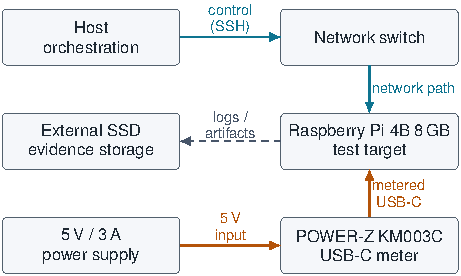
\includegraphics{figures/experiment_setup_schematic.pdf}
\caption{Physical apparatus. A 5-V supply feeds the Raspberry Pi 4B through the POWER-Z KM003C USB-C meter; host orchestration reaches the Pi through the network switch; the external SSD stores evidence artifacts. Teal: network/control; amber: power measurement; dashed: evidence storage. The drawing shows roles and paths only.}
\label{fig:experimentdesign}
\end{figure}
